%%%%%%%%%%%%%%%%%%%%%%
\documentclass{singlecol-new}
%%%%%%%%%%%%%%%%%%%%%%

\usepackage{natbib,stfloats}
\usepackage{mathrsfs}

%
\usepackage{amssymb}
\setcounter{tocdepth}{3}
\usepackage{graphicx}
%\usepackage{url}
\usepackage{amsmath}
\usepackage{amsfonts}
\usepackage{algorithm,algorithmic}
\renewcommand{\algorithmicrequire}{\textbf{Input:}}
\renewcommand{\algorithmicensure}{\textbf{Output:}}
\newcommand{\SWITCH}[1]{\STATE \textbf{switch} (#1)}
\newcommand{\ENDSWITCH}{\STATE \textbf{end switch}}
\newcommand{\CASE}[1]{\STATE \textbf{case} #1\textbf{:} \begin{ALC@g}}
\newcommand{\ENDCASE}{\end{ALC@g}}
\newcommand{\CASELINE}[1]{\STATE \textbf{case} #1\textbf{:} }
\newcommand{\DEFAULT}{\STATE \textbf{default:} \begin{ALC@g}}
\newcommand{\ENDDEFAULT}{\end{ALC@g}}
\newcommand{\DEFAULTLINE}[1]{\STATE \textbf{default:} }
\usepackage{hyperref}

\usepackage{listings}
\usepackage{xcolor}
\usepackage{booktabs}
\usepackage[tight,footnotesize]{subfigure}
%

\def\newblock{\hskip .11em plus .33em minus .07em}

\theoremstyle{TH}{
\newtheorem{lemma}{Lemma}
\newtheorem{theorem}[lemma]{Theorem}
\newtheorem{corrolary}[lemma]{Corrolary}
\newtheorem{conjecture}[lemma]{Conjecture}
\newtheorem{proposition}[lemma]{Proposition}
\newtheorem{claim}[lemma]{Claim}
\newtheorem{stheorem}[lemma]{Wrong Theorem}
%\newtheorem{algorithm}{Algorithm}
}

\theoremstyle{THrm}{
\newtheorem{definition}{Definition}[section]
\newtheorem{question}{Question}[section]
\newtheorem{remark}{Remark}
\newtheorem{scheme}{Scheme}
}

\theoremstyle{THhit}{
\newtheorem{case}{Case}[section]
}

\makeatletter
\def\theequation{\arabic{equation}}

\JOURNALNAME{\TEN{\it Int. J. Web and Grid Services,
Vol. \theVOL, No. \theISSUE, \thePUBYEAR\hfill\thepage}}%

\def\BottomCatch{%
\vskip -10pt
\thispagestyle{empty}%
\begin{table}[b]%
\NINE\begin{tabular*}{\textwidth}{@{\extracolsep{\fill}}lcr@{}}%
\\[-12pt]
Copyright \copyright\ 2019 Inderscience Enterprises Ltd. & &%
\end{tabular*}%
\vskip -10pt%
%\vskip -35pt%
\end{table}%
}

\makeatother

\begin{document}%
%%%%%%%%%%%%%%%%%

\thispagestyle{plain}
\setcounter{page}{1}
\LRH{K. Ma, X. Niu, Z. Yu, and K. Ji}
\RRH{Toward an Aspect-oriented Cache Autoloading Framework with Annotation}
\VOL{19}
\ISSUE{1}
\PUBYEAR{2019}
\BottomCatch
\CLline

\title{Toward an Aspect-oriented Cache Autoloading Framework with Annotation}

\authorA{Kun Ma*\\
*Corresponding author}
%
\affA{Shandong Provincial Key Laboratory of Network Based Intelligent Computing,\\ University of Jinan,\\ Jinan 250022, Shandong, China \\
 E-mail: ise\_mak@ujn.edu.cn, kun.ma.cn@ieee.org\\
*Corresponding author}
%
\authorB{Xuewei Niu}
\affB{Shandong Provincial Key Laboratory of Network Based Intelligent Computing,\\ University of Jinan,\\ Jinan 250022, Shandong, China \\
E-mail: a@niuxuewei.com}

\authorC{Ziqiang Yu}
\affC{Shandong Provincial Key Laboratory of Network Based Intelligent Computing,\\ University of Jinan,\\ Jinan 250022, Shandong, China \\
E-mail: ise\_yuzq@ujn.edu.cn}

\authorD{Ke Ji}
\affD{Shandong Provincial Key Laboratory of Network Based Intelligent Computing,\\ University of Jinan,\\ Jinan 250022, Shandong, China \\
E-mail: ise\_jik@ujn.edu.cn}

\begin{abstract}
In recent years, researches focus on addressing the query bottleneck issue using data cache in the Internet-of-Things. However, the challenges of this method are how to implement autonomous management of data cache. In this paper, we propose an aspect-oriented cache autoloading framework (ACALFA). The architecture, annotation, expression are introduced to address cache auto loading. There are some features for improving performance, such as load waiting, autoloading, loose coupling, and batch delete of cache. The result of experiments indicated that our approach is nearly 25\% faster than other cache frameworks in the scenario that data size is enormous and concurrency is very high.
\end{abstract}

\KEYWORD{Big Data; Data Cache; Aspect-Oriented Programming; Annotation; Pointcut; Grid Services.}

\REF{to this paper should be made as follows: Ma, K., Niu, X., Yu, Z., and Ji, K. (\thePUBYEAR) `Toward an Aspect-oriented Cache Autoloading Framework with Annotation', {\it Int. J. Web and Grid Services}, Vol. \theVOL, No. \theISSUE, pp.xxx\textendash xxx.}

\begin{bio}
Dr. Kun Ma received his Ph.D degree in Computer Software and Theory from Shandong University, Jinan, Shandong, China, in 2011. He is an Associate Professor in School of Information Science and Engineering, University of Jinan, China. He is the Editor-in-Chief of International Journal of Autonomic Computing, editorial board member of International Journal of Grid and Utility Computing. His research interests include situation awareness of public opinion, data intensive computing, big data management, and other big data processing technology. More information at: http://kunma.net.\vs{9}

\noindent Xuewei Niu received his bachelor degree in Computer Science and Technology from University of Jinan in 2019. His research interests include big data management and stream computing.

\noindent Ziqiang Yu received PhD degree from Shandong University, China. His research interests include streaming data processing, spatio-temporal data querying, and urban computing.

\noindent Ke Ji received PhD degree from Beijing Jiaotong University, China. His current research interests include recommender system, information retrieval and machine learning.

\end{bio}

\maketitle


\section{Introduction}
\label{Introduction}

\subsection{Background}
Internet-of-Things (IoT) \cite{zanella2014internet} devices, connected to each other, will generate large-scale data such as weather monitoring data over a relatively short period of time. The real-time IoT data also brings significant challenges for data access and storage \cite{kaisler2013big}. For an optimization, the content routers such as Machine-to-Machine (M2M) gateways in the Internet can cache these results without relaying user requests all the way to data sources. The idea is similar to Content Delivery Network (CDN) of Web pages and multimedia files. However, these systems face cache penetration in the case of high concurrency \cite{nishtala2013scaling}.

In computing, cache is a software component that stores data in memory so that future requests for that data can be served faster. A cache hit occurs reducing server response time when the requested data can be found in a cache, while a cache miss occurs when it cannot \cite{ma2017segment}. There are many examples of caches such as the cache based on browser, the cache based on CDN \cite{manjhi2005finding} and the cache based on applications \cite{wu2011characterization}. Because of performance bottlenecks from queries on Relative Database Management Systems (RDBMSs), it is now common to deploy a memory cache server in conjunction with a database to improve access performance \cite{ma2017column}.

There are a lot of caches, but they all have some shortcomings. Current cache frameworks have some shortcomings. First, their expire policies have not particular optimization for the data that high-frequent access or need a long time to be processed. When the data concentrated is expired, a cache avalanche issue occurred, in case all requests foster together. This case might lead to the instability of the server \cite{ma2017column}. Second, cache logic and business logic are tightly coupled. It leads to cumbersome cache operations and is difficult for developers to maintain the cache data. Third, the cache may cause namespace conflict using distributed key-value database like Redis cluster.

\subsection{Contributions}
In this paper, we propose an aspect-oriented cache auto loading framework with annotation (ACALFA for short). Contributions of our cache framework are concluded as follows.

\begin{itemize}
  \item Avoid cache breakdown and cache penetration using load waiting and autoloading. Autoloading can implement hot-spot data pre-loading. The cache work because the data can be obtained from memory and cut down the read back of source. To further reduce the read back of source, we can make the hot-spot data lurk in memory constantly and update it regularly. Moreover, the data that need to a long time to process also benefit from this strategy, system can load them before peak coming. Load waiting can reduce the server pressure when load data from database. Once the cache miss, there are many requests flowing into the database, but for the same data. Load waiting strategy select a leader to request the data, others wait until the data are provided by the leader.
  \item Loose coupling of business and cache logic using AOP. The purpose of AOP is proposed to decrease the costs of cache maintenance.
  \item Batch delete of cache. It is inevitable that it leads the inconsistency of physical database and cache data. It is difficult to restore the key of the related cache by programs if the query statement is involved. Therefore, the precise batch delete of cache is proposed using hash tables. When this cache need to be removed, the system will remove the record of corresponding hash table directly.
\end{itemize}

\subsection{Organization}
The remainder of the paper is organized as follows. The current work of cache framework is discussed in Section \ref{RelatedWork}. In Section \ref{Framework}, aspect-oriented cache autoloading framework with annotation (ACALFA) is proposed. Architecture, annotation, expression of the aspect-oriented cache auto loading framework are introduced. In Section \ref{Experiments}, the response time, cache improvement and pressure experiments show that our framework are effective and efficient. Brief conclusions and future research directions are outlined in the last section.


\section{Related Work}
\label{RelatedWork}

\subsection{Cache Framework}
Caching of data with weak consistency can achieve transparency. Weak consistency of caching of data leads to the transparency of using. Typically, in-memory caching of data is periodically refreshed. There are different kinds of cache, namely the browser cache \cite{davison2001web}, proxy caching \cite{kumar2008new}, Content Delivery Network (CDN) cache \cite{vakali2003content}, and cache at server level \cite{ma2017column}. Browser cache contains records of every item viewed or downloaded while Internet surfing in local storage \cite{mookerjee2002analysis}. For example, CachePortal \cite{candan2001enabling} is to enable caching of dynamic contents generated by data-driven Web applications. It relies on timestamps and HTTP logs with weak time-lagged consistency. Proxy caching is a feature of proxy servers that stores content on the proxy server itself for web users \cite{kumar2008new}. It can store documents and directly serve requests for them in the network, thereby avoiding repeated traffic to web servers. Compared with proxy caching, CDN has a distributed architecture with low latency \cite{vakali2003content}. The disadvantage of CDN cache is that excessive consumption of resources due to continuous analysis. Both proxy caching and CDN addressed the issues that local cache cannot. Cache at server level is often the culprit of confusion and frustration when it comes to performing dynamic updates.

Recently, there are some new cache frameworks such as the integration of RDBMSs and in-memory NoSQL. There are some cache products such as Redis \cite{zawodny2009redis}, Memcached \cite{hafeez2017realizing}, and EhCache. In this solution, persist data are stored in RDBMS, and high-frequency data are stored in-memory databases {ma2017column}. Redis is an in-memory data structure store for high concurrency and memory consumption. It supports transactions and different levels of on-disk persistence, and provides high availability automatic partitioning. As an improvement, Memcached is an in-memory key-value store by cache access frequency and cache expired cost \cite{nishtala2013scaling}. It is achieved by the time of the cache analysis by distributed dedicated servers.

There are some optimizations of cache frameworks. For example, the performance of distributed storage with disks is studied \cite{scheuermann1998data}. Another data-aware cache framework (Dache) using MapReduce is proposed \cite{zhao2014dache}. In Dache, tasks submit their intermediate results to the cache manager. A task queries the cache manager before executing the actual computing work. In our paper, we propose a general management framework called ACALFA that supports these caches.

\subsection{Aspect-Oriented Programming}
Aspect-Oriented Programming (AOP) is a programming methodology for separating crosscutting concerns \cite{kiczales2001aspect}. This method encapsulates behaviors that affect multiple classes into reusable modules \cite{ma2013toward}. By weaving rules specified by the developer, aspects are incorporated to form the final system. In this paper, we attempt to use this method to intercept cache events to implement the separation of cache from the business.

The key difference between AOP and other approaches is that AOP provides component and aspect languages with different abstraction and composition mechanisms \cite{pinto2017lara}. A special language processor called an aspect weaver is used to coordinate the co-composition of the aspects and components. Modularized crosscutting concerns are called aspects. An aspect, if it can not be cleanly encapsulated in a generalized procedure. AOP distinguishes between two approaches. Static crosscutting affects the static type signature of a program, whereas dynamic crosscutting allows to intercept a program at well-defined points in its execution trace. After evaluating the flexibility of the monitoring system, we decided to pursue dynamic crosscutting option over ease of implementation.

We adopt aspect-oriented programming techniques to manage the data cache. The capabilities of AOP in terms of isolating the aspect code from the source code of the used server make it a non-invasive caching approach.

\section{Aspect-oriented Cache Auto Loading Framework with Annotation}
\label{Framework}

\subsection{Architecture}

\subsubsection{Overview}

\begin{figure} [htb]
\centering
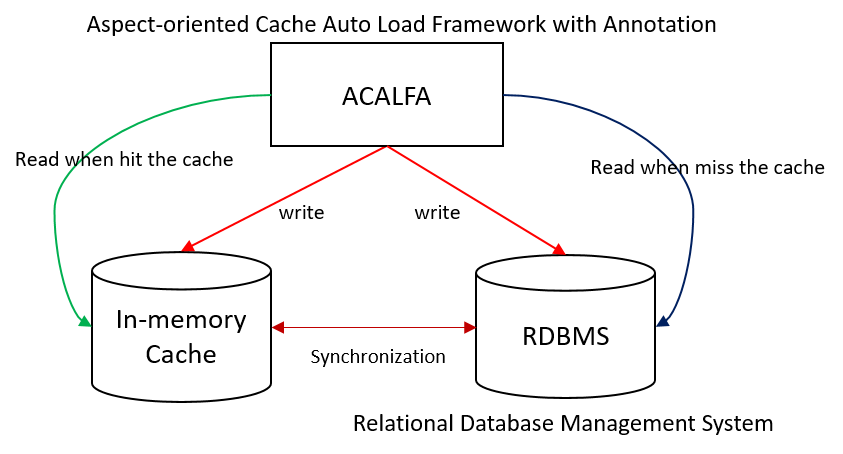
\includegraphics[width=1.0\linewidth]{img/architecture}
\caption{\label{architecture}Architecture of aspect-oriented cache auto loading framework with annotation (ACALFA).}
\end{figure}

Figure \ref{architecture} gives the architecture of our proposed aspect-oriented cache auto loading framework with annotation (ACALFA). ACALFA reads data from in-memory database when it hits the cache, while reads data from relational database management system (RDBMS) when it misses the cache. ACALFA writes data to both in-memory cache and RDBMS. They synchronize the data with each other. This framework is used to reduce the load of reading/writing service of big data applications. Load waiting and auto loading strategy is achieved by decreasing the concurrency number of read back of source RDBMS.

\begin{figure} [htb]
\centering
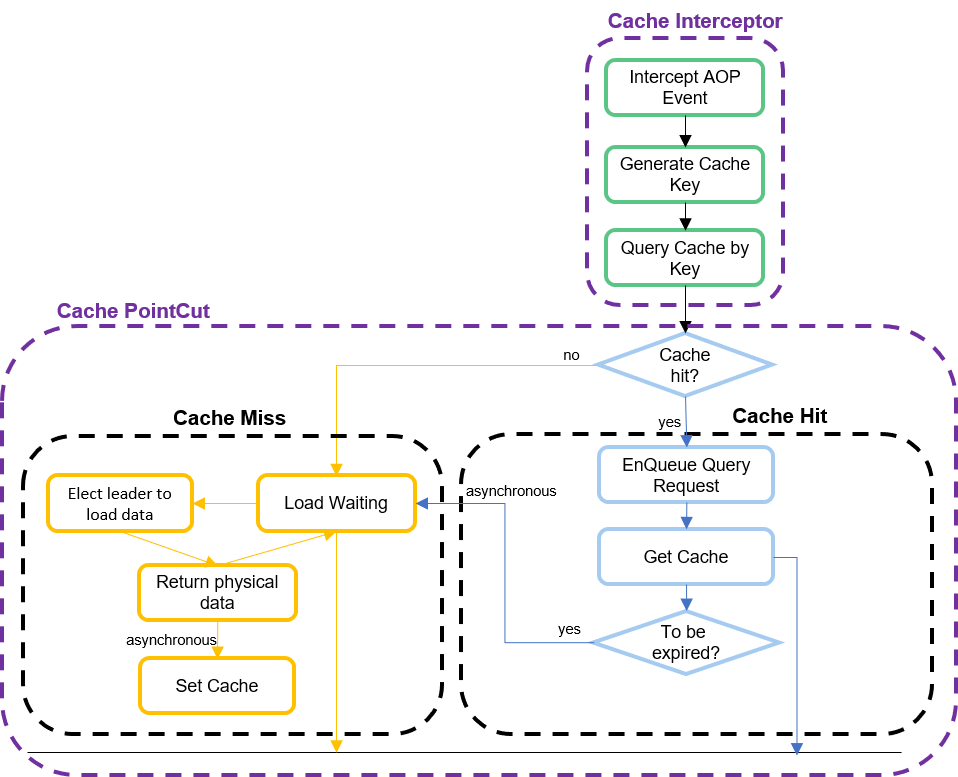
\includegraphics[width=1.0\linewidth]{img/process}
\caption{\label{process}Data processing of aspect-oriented cache auto loading framework with annotation (ACALFA).}
\end{figure}

Figure \ref{process} shows the data processing of aspect-oriented cache auto loading framework with annotation (ACALFA). Using aspect-oriented thinking, cache framework is loosely coupled with business and cache logic. Cache interceptor is used to intercept before/after the execution of business method, then generate the cache key by annotation to trigger cache query. Cache entry is triggered by custom cache events and its corresponding handler. Annotation, a form of metadata, provides data about a program that is not part of the program itself. Cache annotation is used to describe the point cut (cache logic) of our cache framework. It includes cache key, expire time, and cache type. The data of the in-memory cache is loaded by a unique cache key. Cache key is created by the expression in annotation dynamically.

\begin{figure} [htb]
\centering
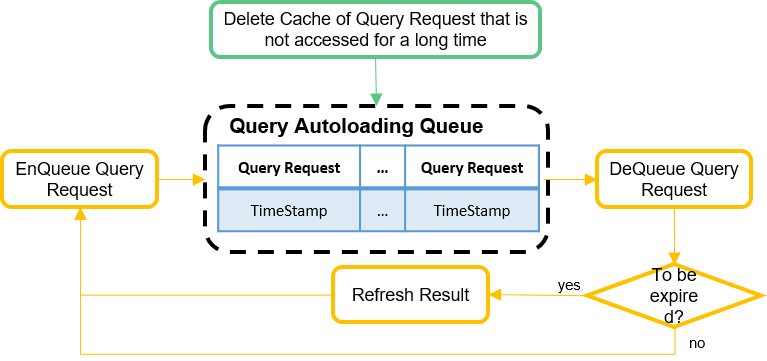
\includegraphics[width=1.0\linewidth]{img/autoloading}
\caption{\label{autoloading}Management of the query autoloading queue.}
\end{figure}

We design the processing of cache hit and miss shown in Figure \ref{process}. When the query hits the query, we put the query request to an autoloading queue for cache self management. If the cache result will be expired, it will trigger an asynchronous update of this cache. Figure \ref{autoloading} shows the management of the query autoloading queue. Cache-context message is recorded in the autoloading queue, including the query request and timestamp. A local thread monitors the autoloading queue to delete the corresponding cache of the query request that is not accessed for a long time. Autoloading queue guarantees the hot spot data is resident in memory. A maximum queue length limit is set to control the capacity.

When the query misses the query, the cache framework will asynchronously elect a leader to load data from physical database. Loading waiting can avoid cache breakdown under high concurrency. That is to say that a large number of query requests with the same key in cache miss will not cause large amount of read back of source physical database.

\subsubsection{Implementation}

ACALFA consists of many components to reduce servers pressure. \textit{Cache interceptor} stores all the cache logic and intercepts all the objects with \textit{@Cache} annotation to implement features, like auto loading, load waiting, etc. The configurations are delivered by the \textit{@Cache} annotation. \textit{Cache pointcut} is a set of join points. It allows where exactly to apply advice, this allows separation of concerns and helps in modularizing business logic. \textit{Cache handler} helps ACALFA determine what is next step, instead implements the specific tasks. It parses cache configurations from \textit{@Cache} annotation by the expression parser. The primary cache configurations are listed below:

\begin{itemize}
    \item \textit{Cache key} defines an unique name to identify them by a expression that could generate a string dynamically according to the parameters.
    \item \textit{Expire time} informs ACALFA of the time that the cache should be removed. The value would be 120(s) if not specify.
    \item \textit{Is cacheable} is a expression that returns a Boolean value. If false, ACALFA will not cache them even though they has \textit{@Cache} annotation.
    \item \textit{Is autoload} is a expression that returns a Boolean value too. The cache cannot reside in the memory if false.
\end{itemize}

\textit{Autoload handler} is the actual cache executor in ACALFA, including multiple internal tasks and queues. The cache that is about to expire and should be auto loaded is updated by it asynchronously. The details about how to implement them will be described in the following part. \textit{Data helper} works with Data Access Object(DAO) that obtains data from database directly. To prevent excessive traffic from flowing into database server, ACALFA resolves it by implementing a strategy, called load wait, in \textit{Data helper}. \textit{Cache handler} encapsulates the functions to operate cache, for example, \textit{get} and \textit{set} in Redis.


\subsubsection{Load Waiting Strategy}

\begin{figure} [htb]
\centering
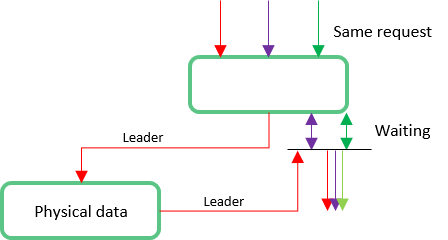
\includegraphics[width=0.8\linewidth]{img/loadwaiting}
\caption{\label{loadwaiting}Data processing of load waiting strategy.}
\end{figure}

Load waiting strategy is used to prevent multiple requests for requesting same data from the physical database at the same time. It is a kind of avoiding of resource wasting. There are mass of traffic flows into database server within a short time once hot-spot data missed. Load waiting selects a leader to get data from database by \textit{Data helper}, instead allows all requests to access to database. Others will be suspended until the leader returns the data. The method to determine which is the same request is by the \textit{Cache key} field that is set in the \textit{@Cache} annotation. Figure \ref{loadwaiting} shows the process of load waiting strategy.

The load waiting strategy algorithm is shown in Algorithm \ref{loadwaitingalg}. \textit{Processing} is a hash map that stores processing requests with different \textit{cache key}. The framework try to get request object from \textit{Processing} hash map by \textit{cache key}. Generally speaking, ACALFA considers this is a new type of request and selects a first arrived request as the leader if returns null. On the contrary, others are waiting until the leader inform them that it is ready for returning values for them.

\begin{algorithm}
\caption{Load waiting strategy algorithm \textit{loadwaiting}}
\label{loadwaitingalg}
\begin{algorithmic}[1]
\REQUIRE ~~\\
  String cacheKey;\\
  Map hashMap;
\ENSURE ~~\\

\STATE Processing processing = hashMap.get(cacheKey);
\IF{processing == null}
\STATE Processing newProcessing = new Processing();
\STATE Processing \_processing = HashMap.putIfAbsent(cacheKey, newProcessing);
\IF{null != \_processing}
\STATE processing = \_processing
\ENDIF
\ENDIF

\IF{processing == null}
\STATE doRequest(newProcessing)
\STATE newProcessing.setFirstFinish(TRUE);
\STATE hashMap.remove(cacheKey);
\STATE newProcessing.notifyAll();
\ELSE
\STATE waitUntilLeaderGotData(processing);
\ENDIF


\RETURN

\medskip

\end{algorithmic}
\end{algorithm}

\subsubsection{Auto Loading Strategy}
In general, developer should preset an expired time for every type of cache. However, the time limit is not suitable for the hot-spot or time-consuming data, especially when traffic peak comes. The cache management system has to load the data from database once cache missed, which may cause response slow, even the server inaccessible. Therefore, to resolve it ACALFA applies a method, called auto loading, that allows those type of data to reside in the memory until they are no longer accessed frequently.

Figure \ref{autoloading} shows the management of the query autoloading queue. \textit{hashTable}, which providing a method called \textit{putIfAbsent} to avoid duplicate tasks and controlling the number of auto loading tasks, is a storage for auto loading assignments. \textit{taskQueue} is taken from \textit{hashTable} by a unified strategy, like LRU. In distributed scenario, the standardized sequence of tasks help the system reduce the read back of source, because others can fetch data from cache rather than database after first server loaded. Auto loading, however, is a double-edged, the system may become unstable if the amount of auto loading tasks were too much or update frequency were too high. Accordingly, a strict inspection should be applied. We assume that $t_n$(ms) is current time, $t_{fr}$(ms) is the first request time, $t_{lr}$(ms) is last request time,  $t_a$(ms) is the average of fetching time, $c$ is the times of cache usage, $t_{to}$ is a preset parameter determining cache time out. There are three main aspects as follow:

\begin{itemize}
    \item Remove if the targeting cache is not requested for a long time. The time of not be requested is get from $t_{nr} = t_n - t_{lr}$, if $t_{nr} > t_{to}$, the task will be discarded.
    \item Remove if efficiency of fetching data from database is high. This may be confused. The intention of auto loading is pre-load the data that cost a lot of time and resources and be accessed frequently. Hence, the data that obtaining efficiency is high should not occupy the space of auto loading. The standard of determination is $c > 100$ and $t_a < 10$.
    \item Remove if usage rate is low. If the cache, which is requested only once within the preset timeout, were added to auto loading queue, that will go against the purposes of auto loading. Therefore, only removing the task that the targeting cache is not requested for a long time is not enough. The usage rate can be get from $r = \frac{c}{t_u}, t_u = {{t_n - t_{fr}}\over{3600000}}$, the meaning of $r$ is how much the cache is requested per hours. If the task has been running for more than 1 hour and the average loading time is less than 1000 ms and $r$ is less than 60, the task will be removed.
\end{itemize}{}

The last part of auto loading is when to refresh the cache. As a pre-loading schema, the cache should be refreshed before expired. For this reason, setting alarm time is valuable. Experiments prove that the default alarm time should be set $t_e - 120$ if $t_e \geq 600$ or $t_e - 60$ if $t_e < 600$, which $t_e$ is a preset parameter determining cache expired time.


\subsubsection{Cache Delete in Batches}
It is difficult to restore or obtain the cache key that need to delete when the query statements are complex, active deletion will hardly complete. In order to manage that, "namespace + hfield + cachekey" schema is proposed. The cache is added string, indicating its namespace, before the cache key, aiming to address conflict in the cache cluster. For active deletion, the key point is that establish a hash table to store the caches that need to be removed together. "hfield" is to identify a unique hash table. Developers can design the deletion granularity on need basis. The process of cache delete in batches is ACALFA intercepts the delete request and inspect whether hfield is set. If hfield is set, ACALFA will delete all the cache that store in corresponding hash table. If not, ACALFA will only delete that cache.

\subsection{Annotation}
Aspects at particular join points enable the modularization of concerns such as cache management that cut across multiple types and objects. We use interceptor as an advice in aspects. Cache pointcuts are put in all DAO classes to implement business hierarchy. Several annotations are designed to describe pointcuts. This framework need intercept the methods with cache annotation and apply cache strategy. There are several annotations, such as \textit{@Cache}, \textit{@ExCache}, \textit{@CacheDeleteKey}, \textit{@CacheDeleteTransactional}, and \textit{@LocalCache}.

\subsubsection{Cache}
\textit{@Cache} that describes the entrance of in-memory caches is one of the most critical annotations. This cache framework will parse the cache configuration in \textit{@Cache} after intercepting this annotation, such as expiration time, the expression of the cache key. When the function of DAO returns data (the data is obtained from the physical database), the framework synchronize the data into the in-memory cache.

\subsubsection{ExCache}
\textit{@ExCache} implements generating multiple caches in one request. It is used to reduce the number of read back of source as long as sorting out the relationship between the cache. The implement of this feature is that framework will determine whether \textit{@Cache} contains \textit{@ExCache} items or not. If yes, framework will generate a new cache according to the configuration.

\subsubsection{CacheDelete}
\textit{@CacheDelete} and \textit{@CacheDeleteKey} implement the cache deleting strategy. \textit{@CacheDelete} is used to remove the cache. \textit{@CacheDeleteKey} is used to generate the cache key that will be removed. The structures are shown as Table \ref{CacheDelete} and \ref{CacheDeleteKey}.

\begin{table}[htb]
\begin{center}
 \caption{\label{CacheDelete}\textit{@CacheDelete} annotation.}
 \begin{tabular}{lll}
 \toprule
Name & Type & Description\\
 \midrule
value & CacheDeleteKey[] & CacheDeleteKey array\\
\bottomrule
 \end{tabular}
\end{center}
\end{table}

\begin{table*}[htb]
\begin{center}
 \caption{\label{CacheDeleteKey}\textit{@CacheDeleteKey} annotation.}
 \begin{tabular}{lll}
 \toprule
Name & Type & Description\\
 \midrule
condition & String & Condition expression and it will return true or false.\\ %The caches are deleted only when its return is true\\
value & String[] & An array saving the cache key expression\\
hfield & String & Expression of hash table field\\
\bottomrule
 \end{tabular}
\end{center}
\end{table*}

\subsection{Expression}
Expression language (EL) is used to generate dynamical variable in the annotation. For example, it can generate the cache key dynamically. There are many types of EL engine, such as Spring EL, Ognl, JavaScript EL. In the case of high performance requirement, Ognl is close to the primitive code. This cache framework provides an abstract class for developers to add user-defined EL.

\begin{itemize}
  \item \textit{Add function} means adding a custom method. In the class of expression parser, there is a hash table which is named \textit{custom functions}. The key of \textit{custom functions} is EL expression, and the value of that is a custom method. In this way, the relationship between expression and custom method is created.
  \item \textit{Get expression value}. Converting an expression to an expected value. The parameters are shown in Table \ref{getExpressionValue}. This function traverses the keys in \textit{custom functions} to register those custom functions.
\end{itemize}

\begin{table}[htb]
\begin{center}
 \caption{\label{getExpressionValue}Parameters of getExpressionValue.}
 \begin{tabular}{ll}
 \toprule
Name & Description\\
 \midrule
arguments & Parameters of intercepted method\\
retVal & Return value of intercepted method\\
hasRetVal & reVal is required or not\\
valueType & Return type of intercepted method\\
\bottomrule
 \end{tabular}
\end{center}
\end{table}

\section{Experiments}
\label{Experiments}

\subsection{Experiment Setup}
Three experiments are designed to illustrate the ACALFA performance in high-concurrency scenario. The metrics are response time, resource consumption and stability. Response time is for validating the optimization of auto loading, especially for time-consuming tasks and high-frequent business. Resource consumption is for validating the load waiting performance when handling the same requests. Stability testing uses multiple threads to access applications simultaneously to simulate high concurrency. The server with ACALFA is an Intel Core i7 @ 3.40GHz CPU, 16GB memory, and 100Mbps bandwidth, and this server runs a 64-bit Windows 10 with a Java 1.8 64-bit server JVM. Another server with MySQL database runs on Ali ECS Cloud Server: 2 core 2.60GHz Intel Xeon E5-2650 CPU machines with 4 GB RAM, 40GB SSD and 100 Mbps Ethernet. The system is CentOS 6.8 x64. Spring Cache, a well-known cache management framework at j2ee, will be compared with ACALFA for performance. The dataset, the structure is shown in Table \ref{VTS}, is selected 4,000 records randomly from a voting system.

\begin{table*}[htb]
\begin{center}
 \caption{\label{VTS}Voting Table Structure.}
 \begin{tabular}{lll}
 \toprule
    Field & Type & Description\\
 \midrule
    id & INT & primary key\\
    candidate\_id & INT & candidate identification\\
    voter\_id & INT & voter identification\\
    score & INT & candidate scores between 1, 100\\
\bottomrule
 \end{tabular}
\end{center}
\end{table*}

\subsection{Response Time}

We set up six experiments to test the ACALFA effect. Cache expired time we set was 120s and enabled auto loading and load waiting for ACALFA. Exp1, exp3 and exp5 used ACALFA, on the contrary, others used Spring Cache. The experiment sets are as follow:

\begin{itemize}
    \item Exp1 \& Exp2: The resources that will be requested were not in cache. Therefore, the frameworks should fetch data from database.
    \item Exp3 \& Exp4: The response time when cache hit.
    \item Exp5 \& Exp6: After exp1 and exp2 120s, in other words, cache expired, we send requests again for validating the effect of auto loading.
\end{itemize}

\begin{figure} [htb]
    \centering
    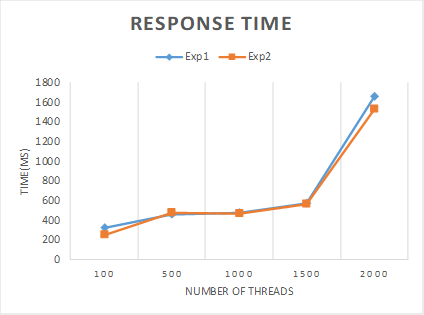
\includegraphics[width=1\linewidth]{img/exp1-2.png}
    \caption{Response time of Exp1 and Exp2}
    \label{exp1-2}
\end{figure}

\begin{figure} [htb]
    \centering
    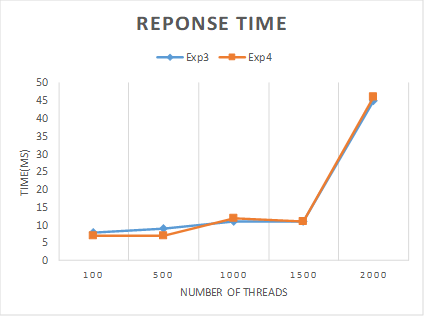
\includegraphics[width=1\linewidth]{img/exp3-4.png}
    \caption{Response time of Exp3 and Exp4}
    \label{exp3-4}
\end{figure}

\begin{figure} [htb]
    \centering
    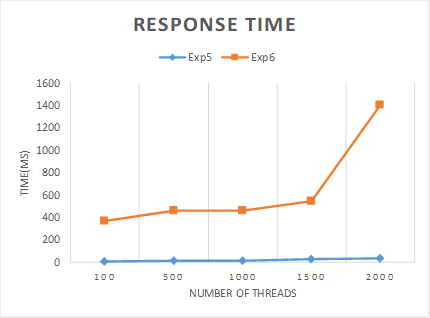
\includegraphics[width=1\linewidth]{img/exp5-6.png}
    \caption{Response time of Exp5 and Exp6}
    \label{exp5-6}
\end{figure}

We use the 90th percentile response time for performance measurement. Figure \ref{exp1-2} and figure \ref{exp3-4} shows the response time is increasing with the increase of number of threads. The performance of two cache management systems when cache miss or cache hit is same roughly. Figure \ref{exp5-6}, however, shows vast difference between ACALFA with auto loading and Spring Cache. The reason is obviously: ACALFA will reload data when the cache is going to expire, but Spring Cache can't. According to this range of experiments, we found auto loading is suited to the hot-spot data and has better cache effects for the more time-consuming or more frequent data.

\subsection{Resource Consumption}

Resource consumption experiment is set for validating the load wait performance. Therefore, the cache is disabled and the query statement is changed to join two tables for increasing cpu usage. There are 30 threads and request 10 times repeatedly. The CPU usage is shown in figure \ref{resource}. From results, CPU usage of non-load-wait lasted for a long time in 100\%. However, ACALFA selected a leader to fetch data in each round of request to reduce the CPU consumption. When elapsed time is more than 30 seconds, the CPU usage of ACALFA is higher than Spring Cache as distributing the data of leader will consume some times. But the most important thing is ACALFA keeps the system run stably. According to the results, we found wait-load strategy is effective in cache miss situation. Coordinate with auto-load, ACALFA can deal with complex and high-concurrent scenario well.

\begin{figure} [htb]
    \centering
    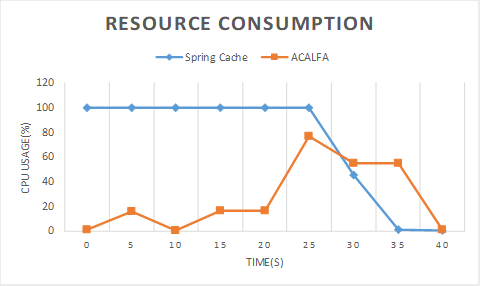
\includegraphics[width=1\linewidth]{img/resource.png}
    \caption{CPU usage of performing the select statement}
    \label{resource}
\end{figure}

\subsection{Pressure Test}

 \begin{figure}
     \centering
     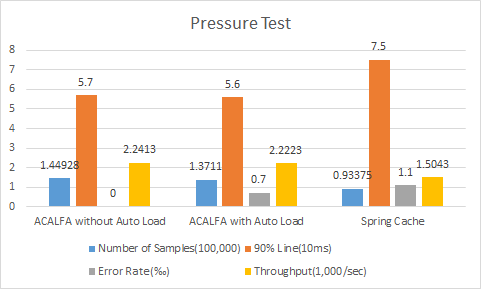
\includegraphics[width=1\linewidth]{img/pressuretest.png}
     \caption{Pressure with different methods}
     \label{pressuretest}
 \end{figure}

 The pressure test is getting access to a page repeatedly within one minute in order to test the stability of ACALFA in high concurrency. We used 100 threads to simulate 100 users for requesting the targeting page simultaneously. We can infer the system availability and response speed from the report. The query statement is same as resource consumption experiment. We can learn ACALFA response is 25\% faster than Spring Cache, processing speed is 48\% faster and stability has improved 36\% from above figure \ref{pressuretest}.

\section{Conclusions}
\label{Conclusions}

The purpose of a cache is to duplicate frequently accessed or important data in such a way that it can be accessed very fast and close to where it is needed. In the big data era, caching generally moves data from a low cost. This paper introduces an aspect-oriented cache auto loading framework with annotation. Several experiments are illustrated that our cache framework has a good effect on the complex business with high concurrency. In the future work, memory resource cost will be optimized to increase cache hit ratio.

\section{Future Work}
\label{futurework}

In the future work, we are going to look for an algorithm to track hot-spot data automatically according to real-time data, instead track them by Annotation. Besides, how to promote cache performance is still a heart of matter to address, like enhancing distributed ability, adding auto-load priority to make sure the important data can be accessed anytime even in the heavy-load environment.


\section*{Acknowledgement}
This work was supported by the National Natural Science Foundation of China (61772231), the Shandong Provincial Natural Science Foundation (ZR2017MF025), the Shandong Provincial Key R\&D Program of China (2018CXGC0706), the Science and Technology Program of University of Jinan (XKY1734 \& XKY1828), and the Project of Shandong Provincial Social Science Program (18CHLJ39).


%%%%%%%%%%%%%%%%%%%%%%%%%%%%%%%%%%%%%%%%%%%%%%%%%%%%%%%%%%%%%%%%%%%%%%%%%%%%%%%%%%%%%

%\bibliography{ijmso}
%\bibliographystyle{unsrt}
%\bibliographystyle{alpha}

\bibliography{mybibtex}
\bibliographystyle{unsrt}

\end{document}
